\chapter{O-MCTS}
\label{sec:planning}

%\todo{hieronder: Dit is onze contributie, ``a novel algorithm'', ``key
%insight'', ``main objective''}
%\todo{Wat gaan we doen: herhalen main objective, teruggrijpen op background en
%introductie}

In order to simulate the use of subgoals, we will introduce planning over
options in MCTS. Planning over options is traditionally done by
applying Q-learning to a set of options instead of the set of actions
\cite{sutton1999between}. Q-learning learns the transition and reward for each
state, but as game complexity increases, the state space grows as well,
increasing Q-learning's memory usage and computation time immensely. In this
chapter we introduce \emph{option Monte Carlo tree search (O-MCTS)}, a novel
algorithm that plans over options using MCTS, enabling the use of options in
complex MDPs.  The resulting algorithm achieves higher scores on complex games
that have several sub-goals than traditional MCTS.

Generally, O-MCTS works as follows: like in MCTS, a tree of states is
built by simulating game plays. In stead of actions, the algorithm chooses
options. When an option is chosen, the actions returned by its policy are used
to build the tree. When an option is finished, a new option has to be chosen.
This enables the tree to branch on that point. This chapter describes in detail
how this process works.

%\todo{How to combine options with MCTS - what problems (challenges) occur?}
In normal MCTS, an action is represented by a connection from a state to a next
state. An option spans over several actions, which influences the tree search
method. Furthermore, when many options are defined, the branching factor of the
algorithm increases significantly. This problem will be addressed in the next
chapter, where we will incorporate learning in the algorithm.

\begin{figure}
	\centering
	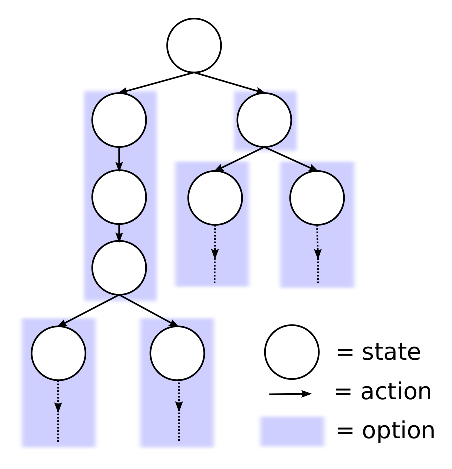
\epsfig{file=includes/omcts.eps, width=.5\columnwidth}
	\caption{The search tree constructed by O-MCTS. In each blue box, one option
	is followed. The arrows represent actions chosen by the option. An arrow
leading to a blue box is an action chosen by the option represented by that box.}
	\label{fig:omcts-tree}
\end{figure}

Traditionally, when a node is at depth $n$, we know that $n$ actions have been
chosen to arrive at that node and the time in that node is $t+n$. If nodes in
O-MCTS would represent options and connections would represent option selection,
this property would be lost, complicating the comparison of different nodes at
the same level in the tree. Therefore, we chose to keep the tree representation
the same: a node represents a state, a connection represents an action. An
option spans several actions and therefore several nodes in the search tree, as
denoted in Figure \ref{fig:omcts-tree}. We introduce a change in the expansion
and selection strategies, which select options, rather than actions. When a node
has an unfinished option, the next node will be created using an action selected
by that option. When a node contains a finished option (meaning that the current
state satisfies its termination condition $\beta$), a new option can be chosen
by the expansion or selection strategy.

Methods exist for automatically generating options \cite{castro2012automatic},
but these are only used on a simple room navigation problem and generating the
options would take learning time which the GVGAI framework does not provide.
Therefore, in this paper options are hand defined. We created a set of options
most of which use the A Star algorithm to navigate the agent towards a specific
game sprite or location \cite{hart1968formal}.

\begin{algorithm}[h]
	\caption{$\mathsf{O-MCTS}(O, r, t, d)$}
	\label{alg:omcts}
	\begin{algorithmic}[1]
		\State $C_{s \in S} \gets \emptyset$ \Comment{$\mathbf{c}_s$ is the set of children nodes of $s$}
		\State $\mathbf{o} \gets \emptyset$ \Comment{$o_s$ will hold the option followed in $s$}
		\While {$time\_taken < t$} \label{alg:omcts:mainloop}
			\State $s \gets r$ \Comment{start from root node}
			\While {$\neg \mathsf{stop}(s, d)$} \label{alg:omcts:innerloop}
				\If{$s \in \beta(o_s)$} \label{alg:omcts:sp} \Comment{if option stops in state $s$}
					\State $\mathbf{p}_s \gets \cup_o (s \in I_{o \in O})$ \Comment{$\mathbf{p}_s$ is available options}
				\Else
					\State $\mathbf{p}_s \gets \{o_s\}$ \Comment{no new option can be selected}
				\EndIf \label{alg:omcts:ep}
				\State $\mathbf{m} \gets \cup_o (o_{s \in \mathbf{c}_s})$ \Comment{set $\mathbf{m}$ to expanded options}
				\If{$\mathbf{p}_s = \mathbf{m}$} \Comment{if all options are expanded}
					\State $s' \gets \max_{c \in \mathbf{c}_s} \mathsf{uct}(s, c)$ \label{alg:omcts:uct} 
						\Comment{child from Eq. \ref{eq:uct}}
					\State $s \gets s'$ \label{alg:omcts:ss} 
						\Comment{continue loop with new node $s'$}
				\Else \label{alg:omcts:sexpand}
					\State $\omega \gets \mathsf{random\_element}(\mathbf{p}_s - \mathbf{m})$ 
					\State $a \gets \mathsf{get\_action}(\omega, s)$ 
					\State $s' \gets \mathsf{expand}(s, a)$ 
						\Comment{create child $s'$ using $a$}
						\State $\mathbf{c}_s \gets \mathbf{c}_s \cup \{s'\}$ \Comment{add $s'$ to $\mathbf{c}_s$}
					\State $o_{s'} \gets \omega$
					\State \textbf{break} \label{alg:omcts:break}
				\EndIf \label{alg:omcts:eexpand}
			\EndWhile
			\State $\delta \gets \mathsf{rollout}(s')$ \label{alg:omcts:rollout}
				\Comment{simulate until $\mathsf{stop}$}
			\State $\mathsf{back\_up}(s', \delta)$ \label{alg:omcts:backup}
				\Comment{save reward to parent nodes}
		\EndWhile
		\State \Return{$\mathsf{get\_action}(\max_{o \in c_r} \mathsf{value}(o), r)$}
	\end{algorithmic}
\end{algorithm}
\begin{figure}
	\centering
	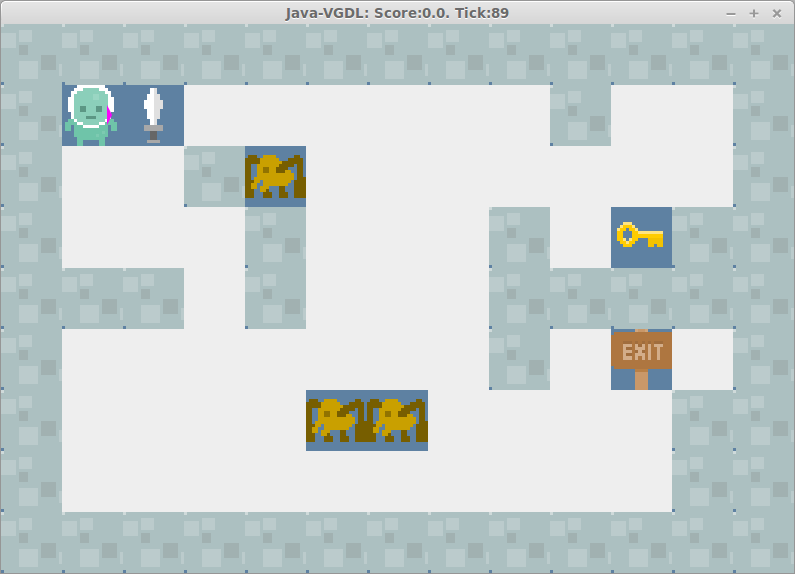
\includegraphics[width=.6\textwidth]{includes/zelda}
	\caption{Visual representation of the game \textit{zelda}.}
	\label{fig:zelda}
\end{figure}

We describe O-MCTS in Algorithm \ref{alg:omcts}. It is invoked with a set of
options $O$, a root node $r$, a maximum runtime $t$ in milliseconds and a
maximum search depth $d$. Two variables are instantiated. $C_s$ is a set of
sets, containing the set of child nodes for each node and $\mathbf{o}$ contains
which option is followed for each node. The main loop starts at line
\ref{alg:omcts:mainloop}, which keeps the algorithm running until time runs out.
The inner loop runs until a node $s$ is reached that meets a stop criterion
defined by the function \textsf{stop}, or a node is expanded into a new node.
In lines \ref{alg:omcts:sp} until \ref{alg:omcts:ep}, $\mathbf{p}_s$ is set to
all options that are available in $s$. If an option has not finished,
$\mathbf{p}_s$ contains only the current option. Otherwise, it contains all the
options $o$ that have state $s$ in their initiation set $I_o$. For example, when
the agent is playing \textit{zelda} (see Figure \ref{fig:zelda} and the current state $s$
shows no NPCs on screen. If there is an option $o$ that goes to NPCs, $I_o$ will
not contain state $s$, because there are no NPCs on screen, rendering $o$
useless in state $s$. $\mathbf{p}_s$ will thus not contain option $o$, since $s$
is not in $o$'s initiation set $I_o$.

Then, the four phases of Figure \ref{fig:mcts} are implemented as follows.  If
the set $\mathbf{p}_s$ is the same as the set of options in the children of $s$,
$m$, i.e. all options have been explored at least once in node $s$, a new node
$s'$ is \emph{selected} by \textsf{uct} In line \ref{alg:omcts:ss}, $s$ is
instantiated with the new node $s'$, continuing the inner loop using this node.
If some options are unexplored in node $s$, it is \emph{expanded} with a random,
currently unexplored option by lines \ref{alg:omcts:sexpand} to
\ref{alg:omcts:eexpand}. After expansion or when the stop criterion is reached,
the tree selection loop is stopped and a \emph{rollout} is done, resulting in
score difference $\delta$. This score difference is \emph{backed up} to the
parent nodes of $s$ using the backup function, after which the tree traversal
restarts with the root node $r$.

A couple of functions are used by Algorithm \ref{alg:omcts}. The function
\textsf{stop} returns true when either the game ends in state $s$ or the maximum
depth is reached in $s$. The function \textsf{get\_action} lets option $o$
choose the best action for the state in node $s$, \textsf{apply\_action} applies
the action to state $s$ in the simulator, returning the resulting state.The
function \textsf{expand} creates a new child node for node $s$ with option $o$.
Typically, the \textsf{rollout} function chooses random actions until
\textsf{stop} returns true, after which the difference in score achieved by the
rollout is returned.  In O-MCTS however, \textsf{rollout} always applies actions
chosen by option $o$ first and applies random actions after $o$ is finished. The
\textsf{back\_up} function traverses the tree through all parents of $s$,
updating their expected value.

When the time is up, the algorithm chooses an option from $c_r$ corresponding to
the child node highest expected value. This option chooses the best
action for the state in the root node and that action is returned. The agent
plays out this action. 

In the next state, the algorithm starts anew by creating a new root node from
this state. Note that O-MCTS returns actions, not options. This way, when an
option would eventually reach a state where the avatar dies, it does not have to
be followed until it is finished. This can be seen as a version of option
interruption as discussed in \cite{sutton1999between}.

We expect that this implementation of MCTS with options enables the algorithm to
create a deeper tree search, looking further ahead and that the usage of options
will enable the algorithm to plan over subgoals. In the experiments chapter we
show results that support our expectations.
